%!TEX root = Paper.tex
% \vspace{-10pt}
\section{Experimental Validation}
\vspace{-0.75em}

    % --iL with different gamma, stacked
    % -- efficiency, 3D
    
    % - Peak efficiency occurs above resonance. This implies the converter is conduction and core loss dominated at resonance when the rms inductor current is maximal.
    
    % - The timings in (\ref{eqn:t1_approx}) and (\ref{eqn:t2_approx}) were verified with a practical prototype as shown in Fig.~\ref{fig:iL_meas}.
    
    % - Maybe mention the `tails' of the measured inductor current?

Testing of the hardware prototype, shown in Fig.~\ref{fig:board}, validated that the approximate phase durations derived in (\ref{eqn:t1_approx}) and (\ref{eqn:t2_approx}) match experimental results both at- and above-resonance (i.e., $\Gamma \leq 1$) as shown in Fig.~\ref{fig:iL_meas}.
Moreover, Fig. \ref{fig:corr_vs_incorr} illustrates up to a 15\% decrease in converter losses when the derived optimal phase durations are used in place of equal phase intervals.
% 19\% increase


Efficiency, $\eta$, was also measured across a range of output current $I_{out}$ and $\Gamma$; Fig.~\ref{fig:eff} illustrates an interpolated contour of these measured efficiencies.
As $\Gamma$ decreases below unity (i.e., $f_{\textrm{sw}}$ increases), the efficiency is maximized in the region $0.5<\Gamma<0.9$. 
This hardware prototype demonstrates that above-resonance operation ($\Gamma<1$) can result in an improved overall efficiency through the significant reduction of conduction losses despite losing ZCS and the increase of switching losses---a conclusion shared by \cite{Rentmeister_COMPEL2018}.
Additionally, the point of peak efficiency appears invariant of load across the range of $\Gamma$.
% A 5:1 FCML with $V_{HI}=200$~V, $L=3.39~\mu$H, $C_0=0.93~\mu$F ($f_{\textrm{sw},\textrm{res}}$)


\begin{figure}[t]
 \vspace{-30pt}
\hspace{-20pt}
\begin{minipage}[H]{0.35\linewidth}
%%%%%%%%%%%%%%%%%%%%%%%%%%%%%%%%%%%%%%%%%%%%%%%%%%%%%%%%%%%%%%%%%%%%%%%%%%
 %   \centering
 %   % 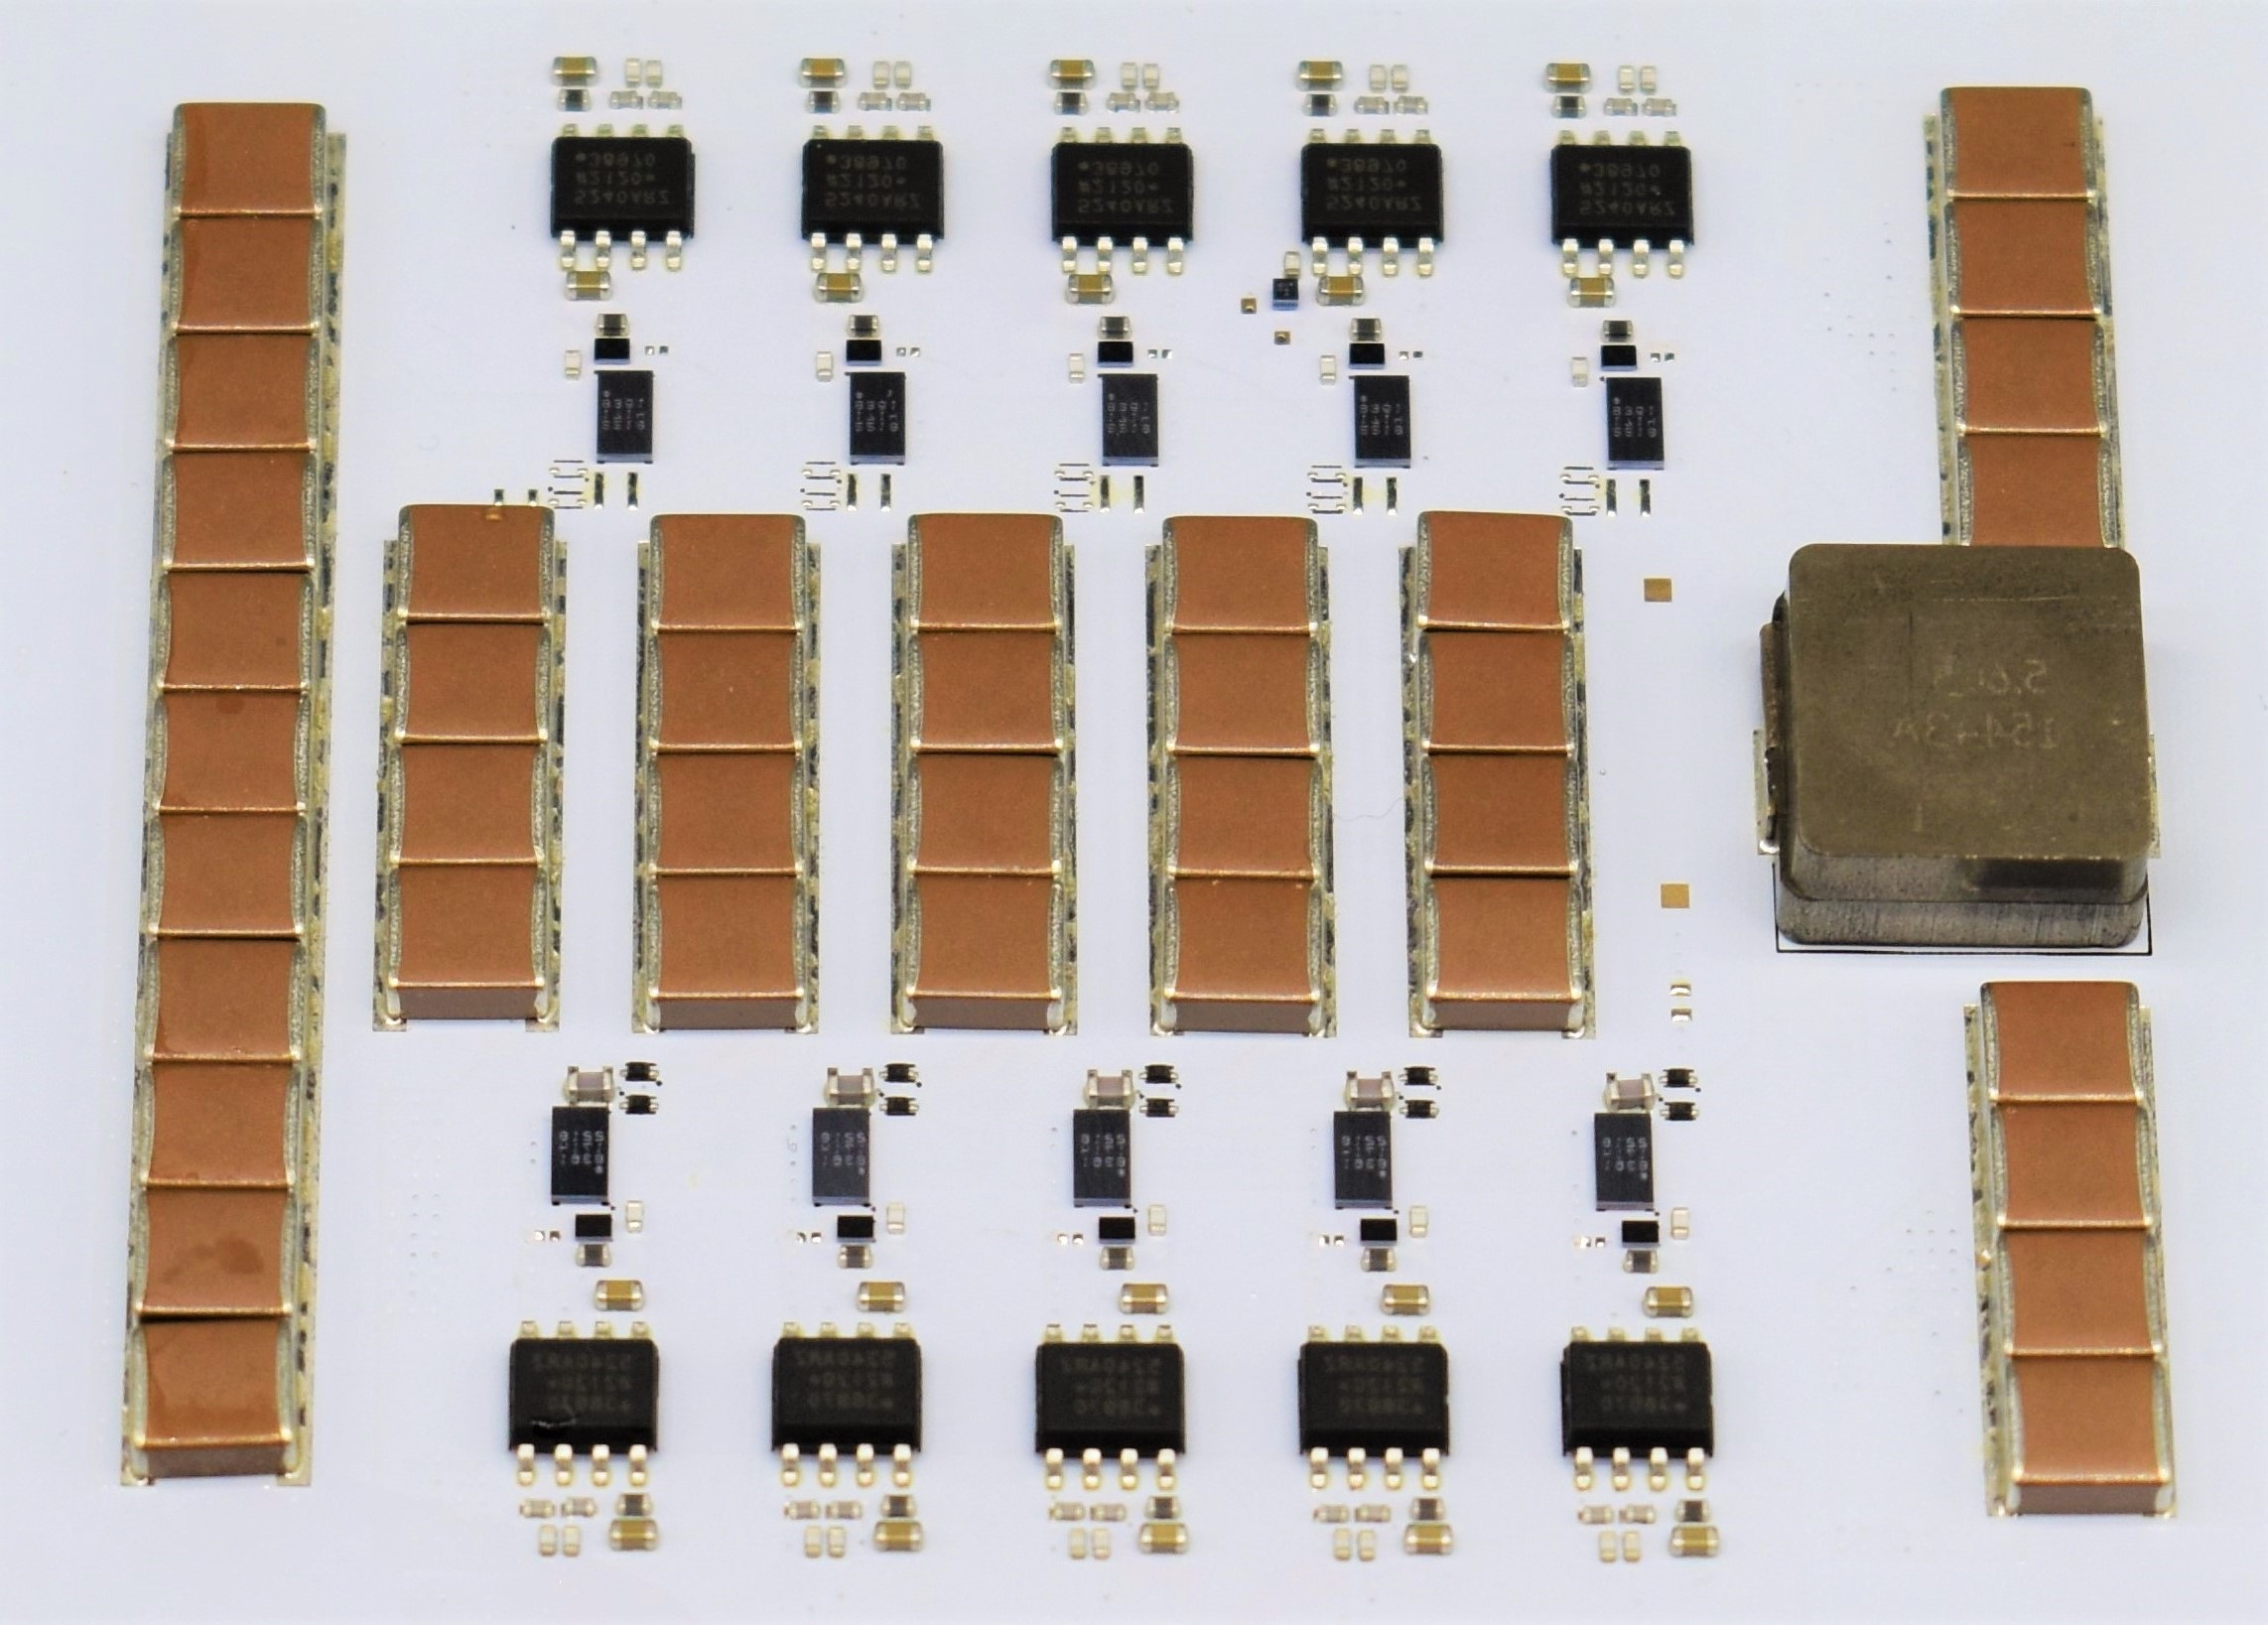
\includegraphics[width=1\linewidth]{Figures/clean_photo_cropped_3.jpg}
 %   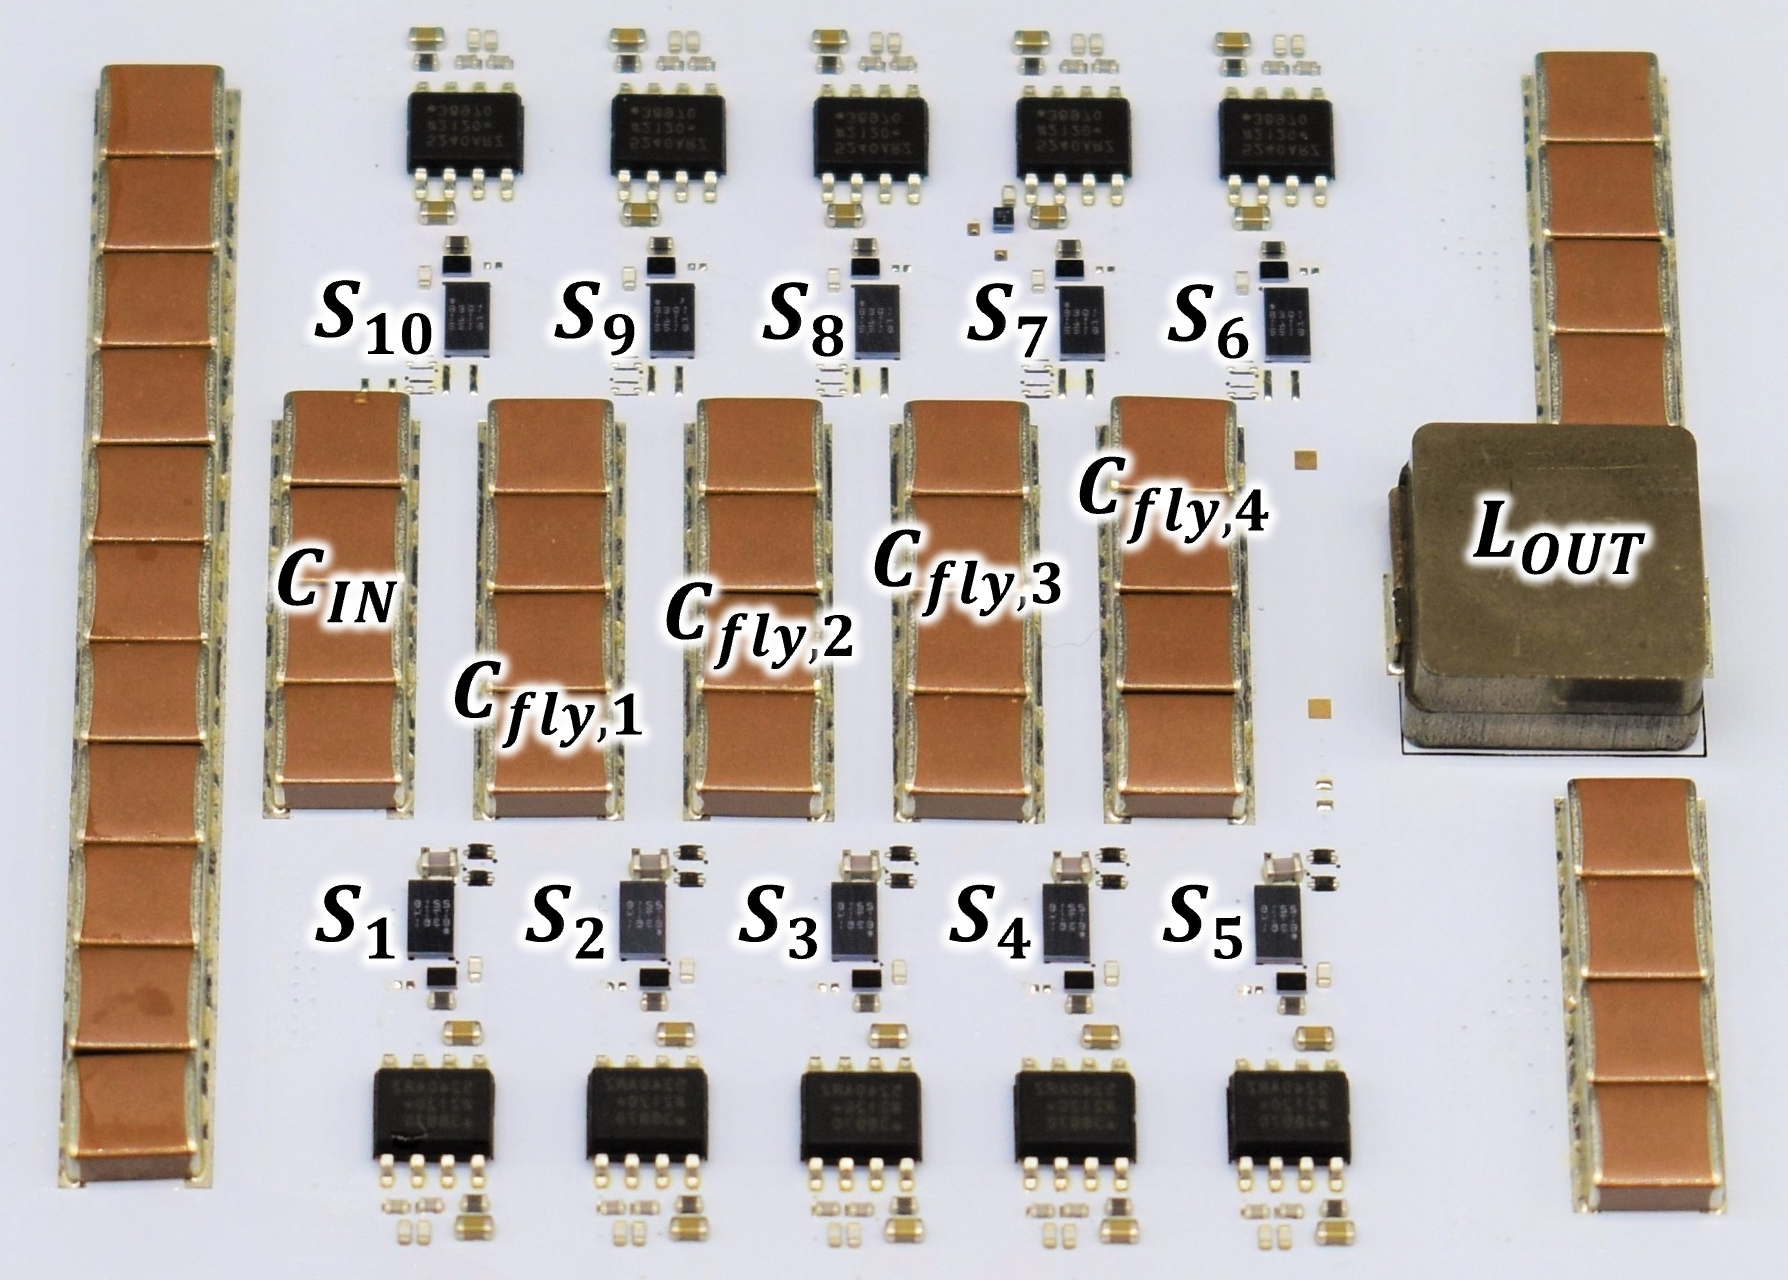
\includegraphics[width=1\linewidth]{Figures/annotated_photo.png}
 %   \caption{Photograph of the constructed 5:1 FCML hardware prototype.}
 %   \label{fig:board}
     \centering
    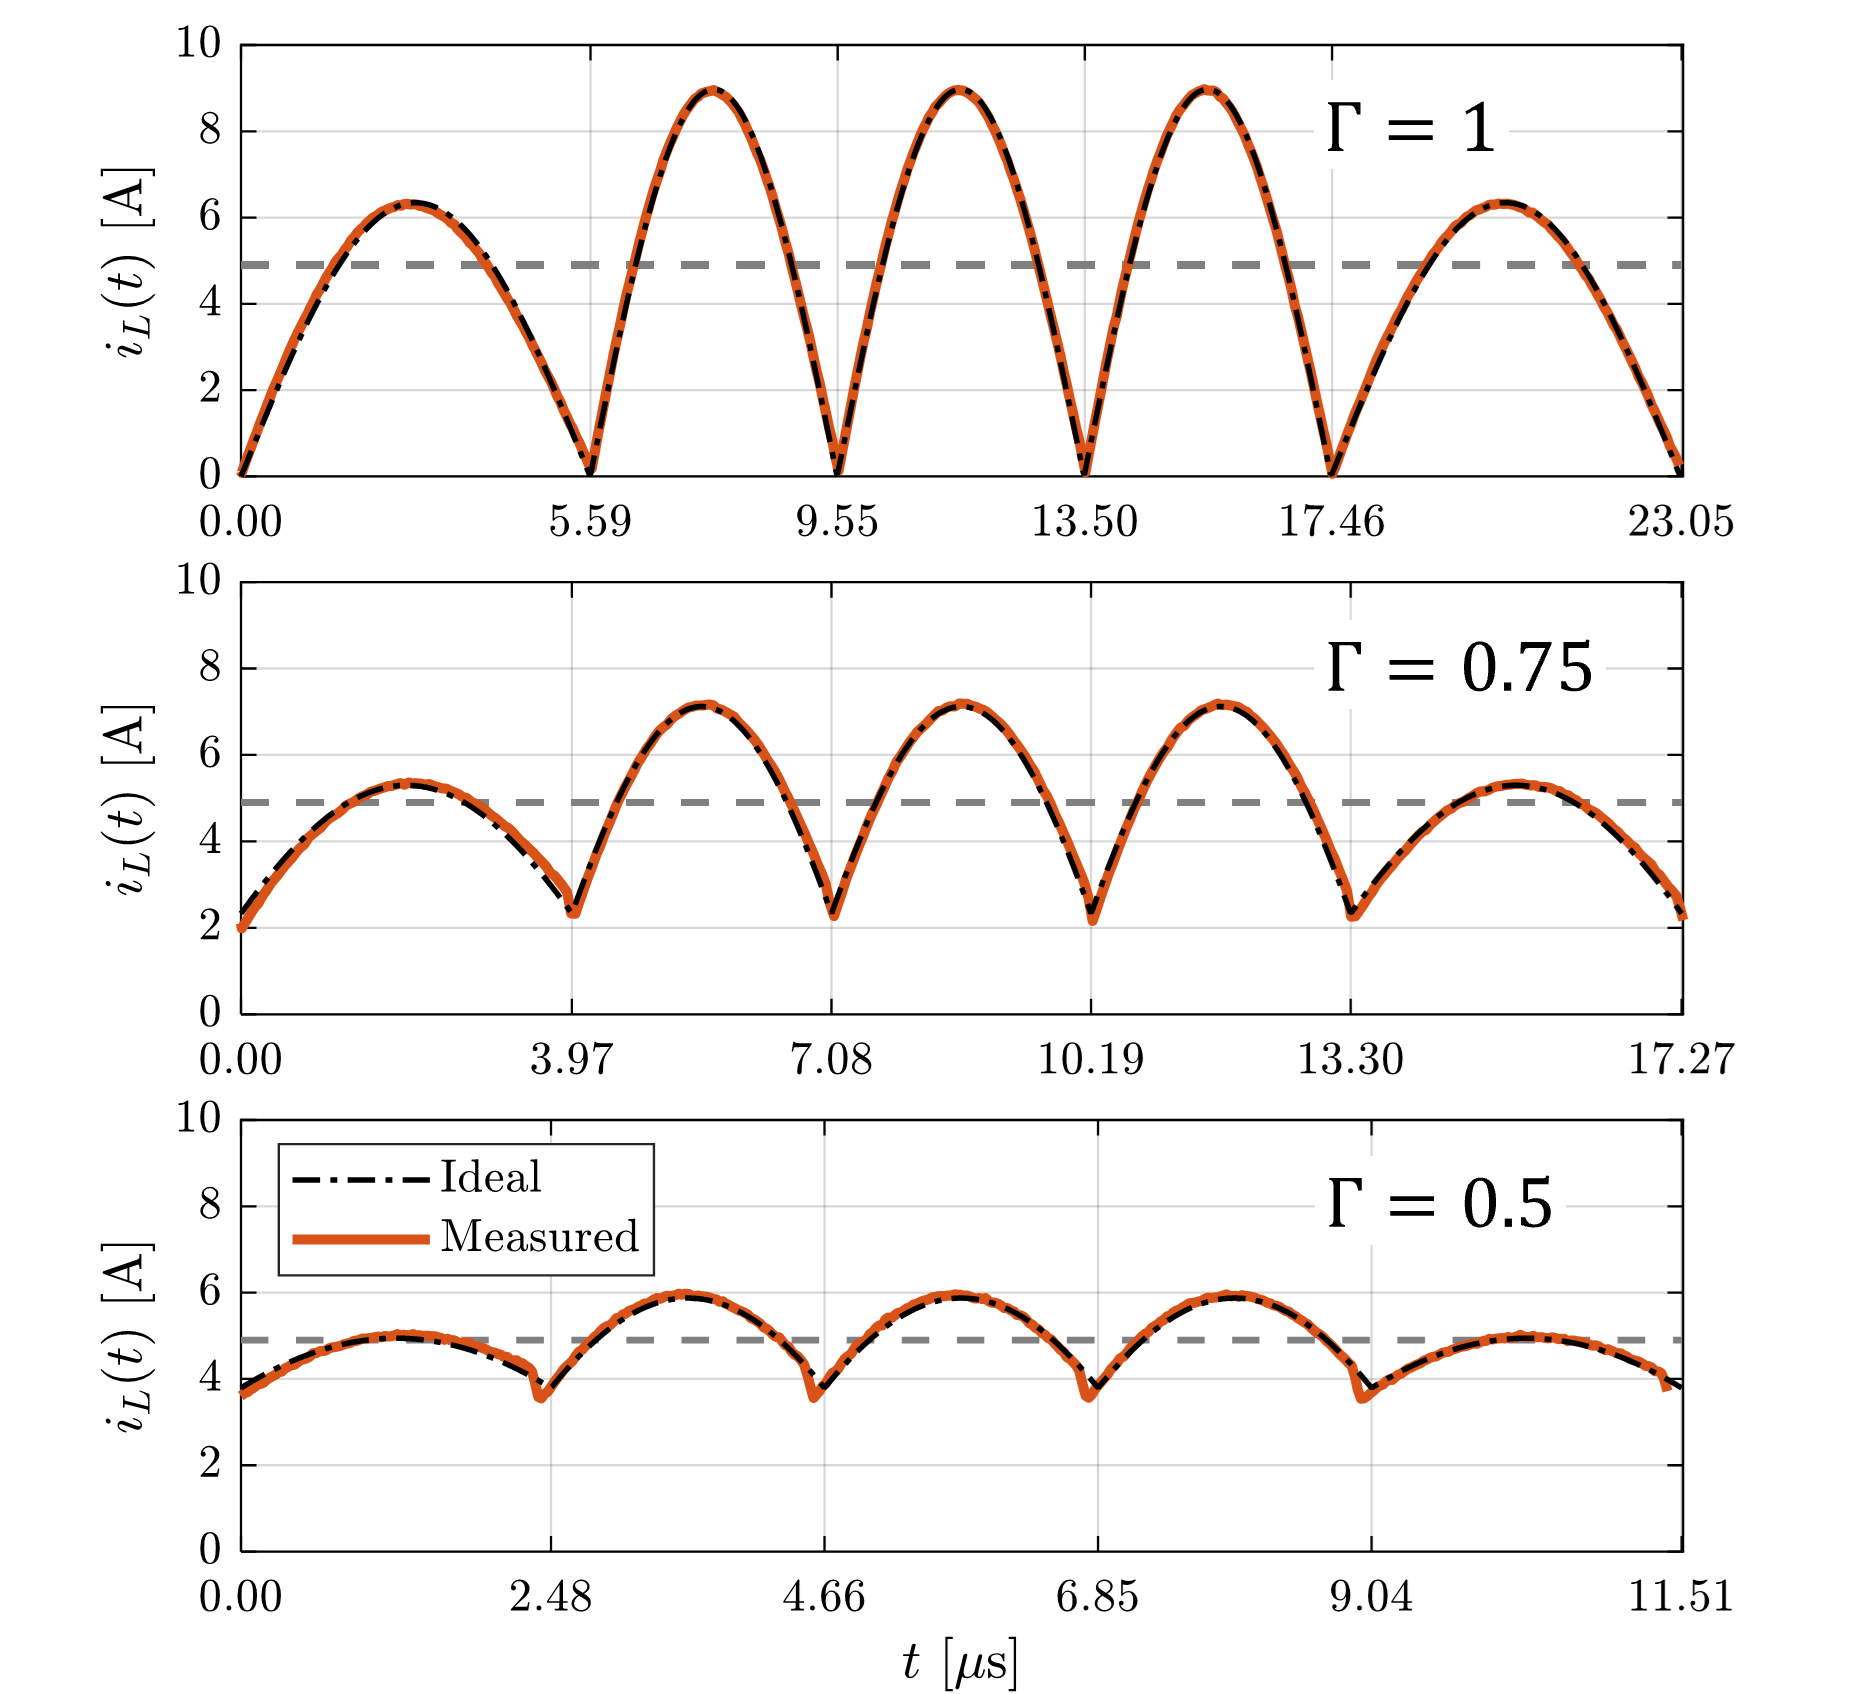
\includegraphics[width=1\linewidth]{Figures/MeasWaveforms_all_a.png}
    \caption{Measured vs ideal inductor current waveforms for various $\Gamma$ ($N=5$, $I_{out}=4.9$~A).}
    \label{fig:iL_meas}
    %%%%%%%%%%%%%%%%%%%%%%%%%%%%%%%%%%%%%%%%%%%%%%%%%%%%%%%%%%%%%%%%%%%%%%%%%%
\end{minipage}
% \hspace{20pt}
\hfill
\begin{minipage}[H]{0.3\linewidth}
%%%%%%%%%%%%%%%%%%%%%%%%%%%%%%%%%%%%%%%%%%%%%%%%%%%%%%%%%%%%%%%%%%%%%%%%%%

  
     \centering
    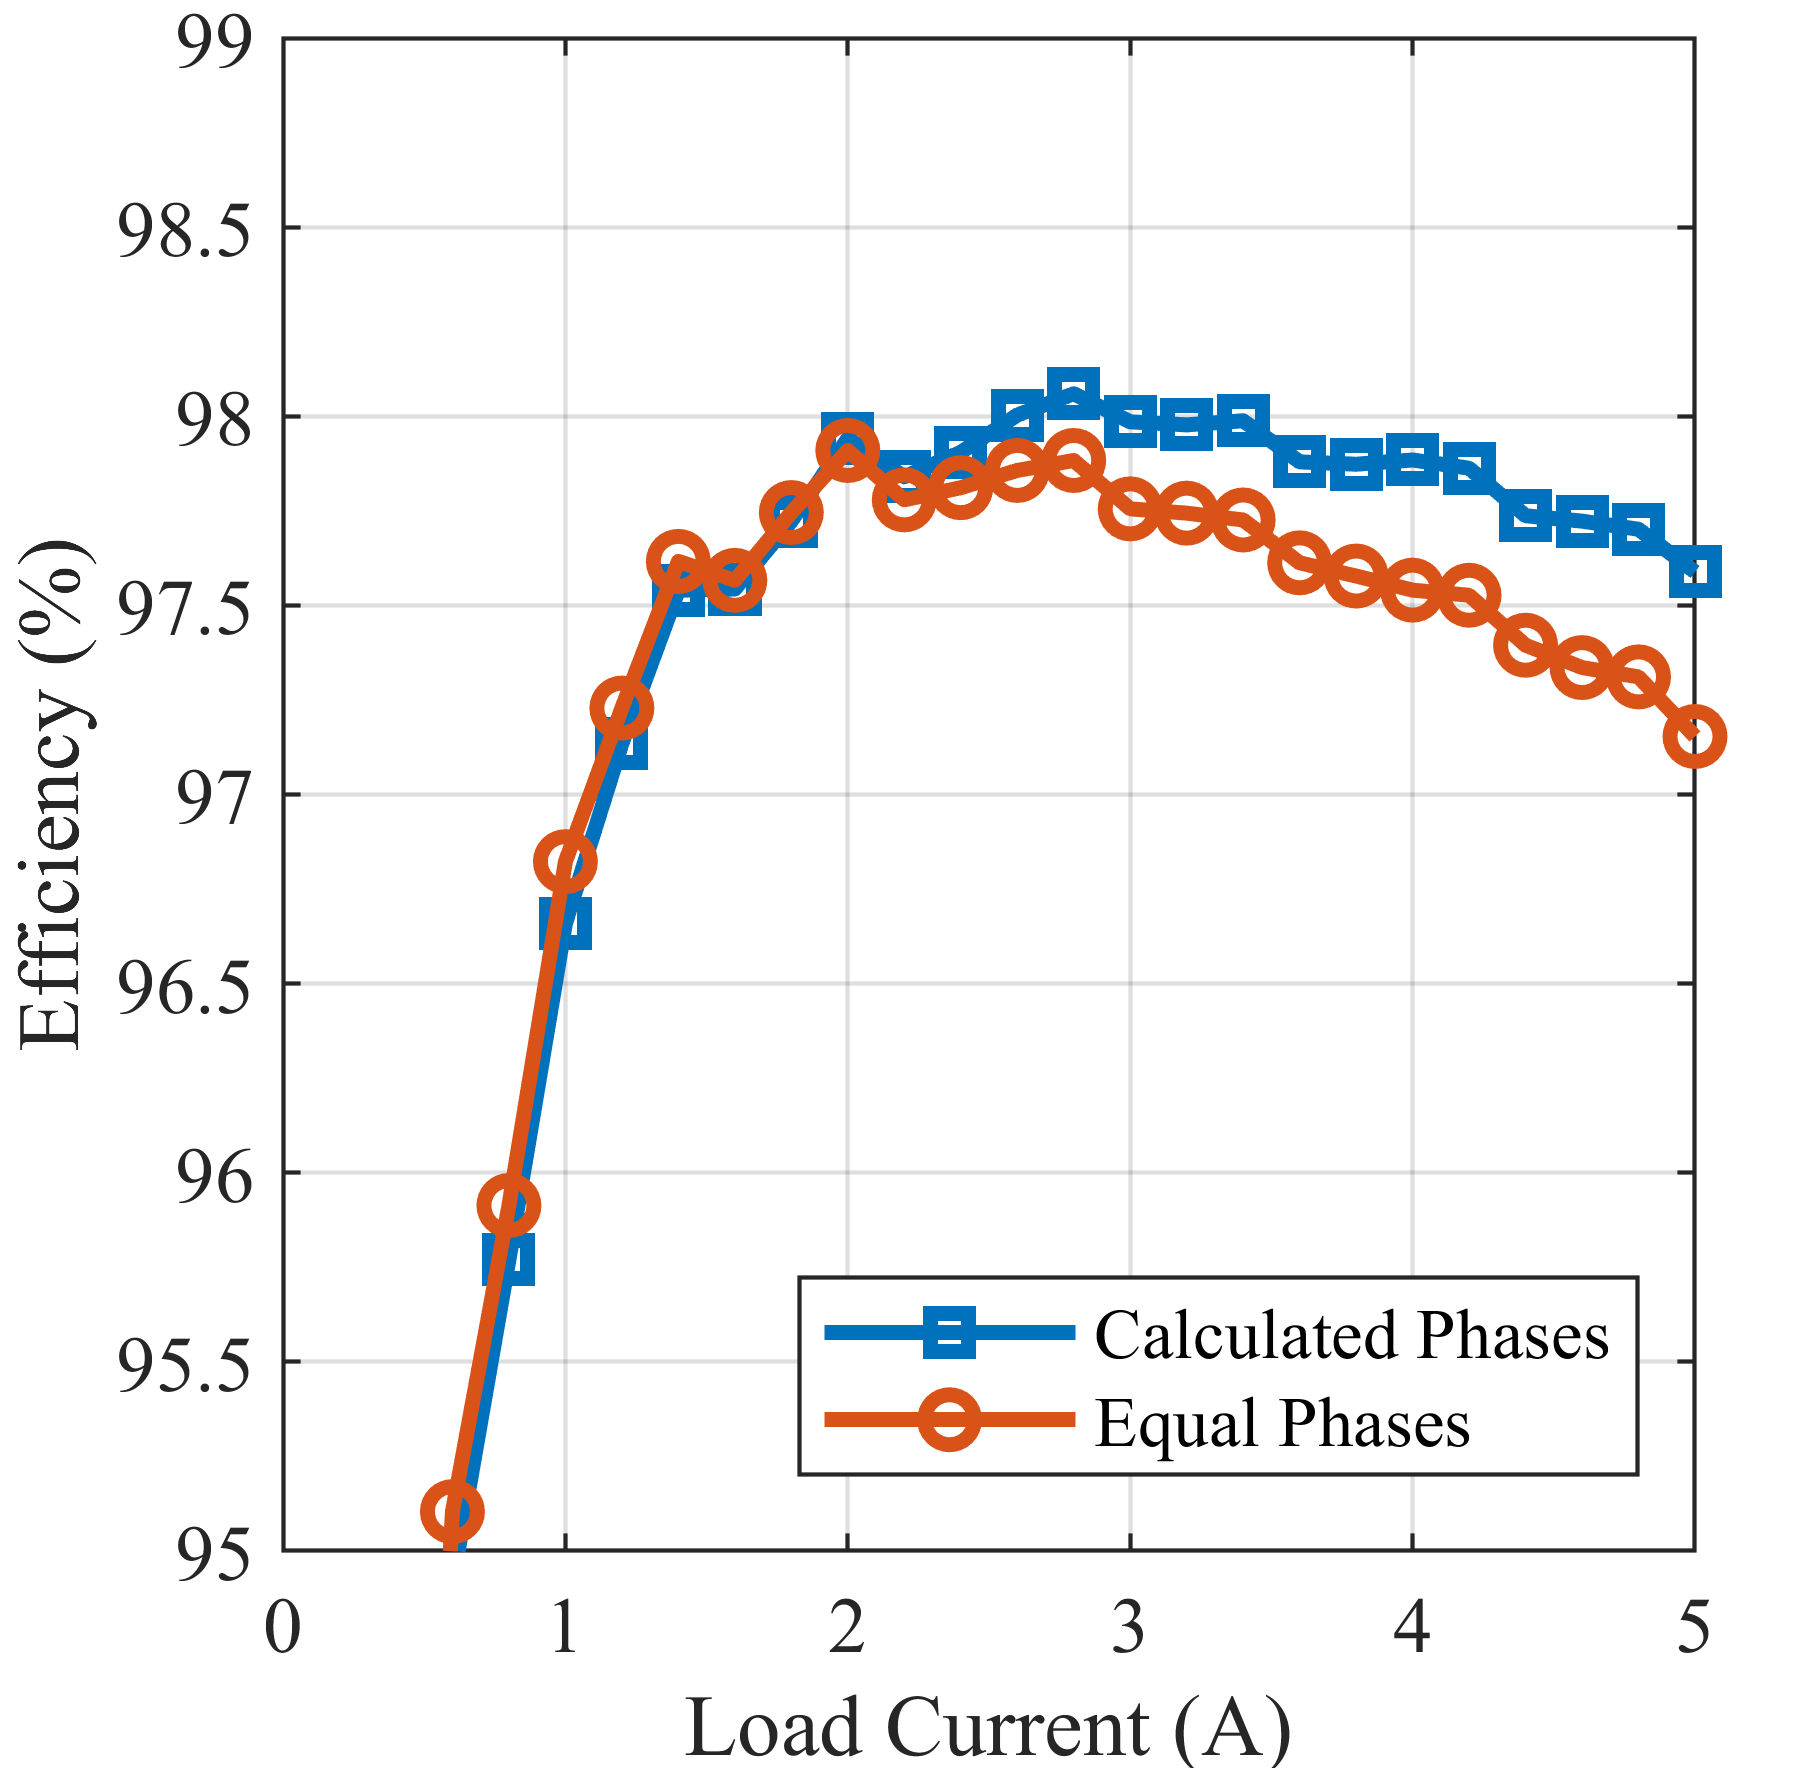
\includegraphics[width=1\linewidth]{Figures/corr_vs_incorr_Eff_vs_load.png}
    \caption{Measured efficiency curves comparing FCML operation using the calculated phase durations, versus setting all phase durations equal in length. The latter sees up to a 19\% increase in losses.}
    \label{fig:corr_vs_incorr}
  
    %%%%%%%%%%%%%%%%%%%%%%%%%%%%%%%%%%%%%%%%%%%%%%%%%%%%%%%%%%%%%%%%%%%%%%%%%%
\end{minipage}
\hfill
\hspace{5pt}
\begin{minipage}[H]{0.35\linewidth}
%%%%%%%%%%%%%%%%%%%%%%%%%%%%%%%%%%%%%%%%%%%%%%%%%%%%%%%%%%%%%%%%%%%%%%%%%%
    \centering
    \vspace{8pt}
    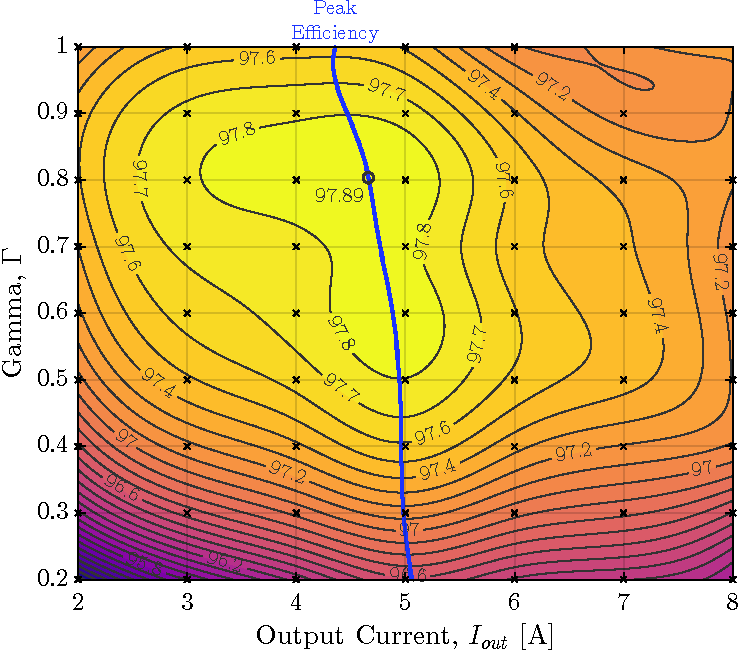
\includegraphics[width=1\linewidth]{Figures/3D_MeasEfficiency_1b.pdf}
    \caption{Measured efficiency contour with swept $I_{out}$ and $\Gamma$. Datapoints located on gridline intersections. $N~=~5$, $V_{HI}~=~200$~V, $L=3.39$\;$\mu$H, $C_0=0.93\;\mu$F ($f_{\textrm{sw},\textrm{res}}=43.4$\;kHz). }
    \label{fig:eff}
    %%%%%%%%%%%%%%%%%%%%%%%%%%%%%%%%%%%%%%%%%%%%%%%%%%%%%%%%%%%%%%%%%%%%%%%%%%
\end{minipage}
\vspace{-10pt}
\end{figure}
